% \section*{Midterm 1 Review}

\renewcommand{\arraystretch}{1.25}

\subsection*{MOSFET Behavior and Models}

\begin{center} 
\begin{tabular}[t]{|c|c|p{60px}|p{275px}|}
\hline
Type & Drawing & Switch Closed & Behavior \\ \hline
 \begin{minipage}[c]{30px} PMOS \end{minipage} & \begin{minipage}[c]{50px} \begin{circuitikz}[american] 
\draw (0, 0) node[pmos, emptycircle] (nmos) {};
\draw (nmos.G) node[left]{$G$};
\draw (nmos.S) node[left]{$S$};
\draw (nmos.D) node[left]{$D$};
\end{circuitikz}
\end{minipage} & 
\begin{minipage}[c]{60px} $V_{GS} \leq -|V_{tp}|$ \end{minipage} &
\begin{minipage}[t]{275px}
\vspace{-15px}
Closed switch when gate voltage $V_G$ is at least $|V_{tp}|$ below source voltage $V_S$ (gate voltage is low). Open switch otherwise.
\end{minipage} \\ \hline
\begin{minipage}[c]{30px} NMOS \end{minipage} & 
\begin{minipage}[c]{50px}
\begin{circuitikz}[american] 
\draw (0, 0) node[nmos] (nmos) {};
\draw (nmos.G) node[left]{$G$};
\draw (nmos.S) node[left]{$S$};
\draw (nmos.D) node[left]{$D$};
\end{circuitikz}
\end{minipage} & 

\begin{minipage}[c]{60px} $V_{GS} \geq |V_{tn}|$ \end{minipage} &

\begin{minipage}[t]{275px}
\vspace{-15px}
Closed switch when gate voltage $V_G$ is at least $V_{tn}$ above source voltage $V_S$ (gate voltage is high). Open switch otherwise.
\end{minipage} \\ \hline
\end{tabular} \end{center}

\begin{center} \begin{tabular}{|c|c|c|c|}
\hline
Type & (Voltage-Controlled) Switch & Resistor-Switch & Resistor-Capacitor-Switch \\ \hline
\begin{minipage}[c]{30px} \vspace{-110px} PMOS \end{minipage}
 & \begin{circuitikz}[scale=0.9]
			\draw (0, -2) node[label=left:$D$] {}
			to[switch, l_= $V_{GS} \leq -|V_{tp}|$, *-] (0,2)
			to[short, -*] ++(0, 0.2)
            node[label=right:$S$] {};;
			\draw (0, 2) -- (-1, 2) to [short, -o] (-1, 2);;
            \draw (-2, 0) to [short, -*] (-2, 0)
                          to [short, -o] (-1, 0) node[label=below:$G$] {}
                          to [open, v^=$V_{GS}$] ++(0, 2);;
			% to[short, -*] ++(0, -2) node[label=left:$G$] {};;
            % \draw (-1, -2) node[label=left:$G$] {};;
			\draw (0, -1.75) to [short, -*, l=$V_{out}$] ++(1,0);;
		\end{circuitikz} & 
        \begin{circuitikz}[scale=0.9]
			\draw (0, -2) node[label=left:$D$] {}
			to[switch,l_= $V_{GS} \leq -|V_{tp}|$, *-] (0,0)
			to[R, l_=$R_{on, P}$, i<=$I_D$] ++(0, 2)
			to[short, -*] ++(0, 0.2) node[label=right:$S$] {};;
            \draw (0, 2) -- (-1, 2) to [short, -o] (-1, 2);;
            \draw (-2, 0) to [short, -*] (-2, 0)
                          to [short, -o] (-1, 0) node[label=below:$G$] {}
                          to [open, v^=$V_{GS}$] ++(0, 2);;

			% \draw (0, 2) -- (-1, 2)
			% to[short, -*] ++(0, -2) node[label=left:$G$] {};;
			\draw (0, -1.75) to [short, -*, l=$V_{out}$] ++(1,0);;
		\end{circuitikz} &
        \begin{circuitikz}[scale=0.9]
			\draw (0, -2) node[label=left:$D$] {}
			to[switch,l_= $V_{GS} \leq -|V_{tp}|$, *-] (0,0)
			to[R, l_=$R_{on, P}$, i<=$I_D$] ++(0, 2)
			to[short, -*] ++(0, 0.2)
            node[label=right:$S$] {};;
			\draw (0, 2) -- (-2, 2);;
			\draw (-2, 0) to[short, -*] ++(0, 0) node[label=left:$G$] {} to[C, l_=$C_{GS}$, v^=$V_{GS}$] ++(0, 2);;
			\draw (0, -1.75) to [short, -*, l=$V_{out}$] ++(1,0);;
		\end{circuitikz} \\ \hline

\begin{minipage}[c]{30px} \vspace{-110px} NMOS \end{minipage}
 & \begin{circuitikz}[scale=0.9]
            \draw (0,-2)
            to[switch,l_= $V_{GS} \geq V_{tn}$]
            (0,2) to[short, -*] ++(0,0)
            node[label=left:$D$] {};;
            % \draw (0,-2) -- (-1,-2)
            % to[short, -*] ++(0,2) node[label=left:$G$] {};;
            \draw (0, -2) -- (-1, -2) to [short, -o] (-1, -2);;
            \draw (-2, 0) to [short, -*] (-2, 0)
                          to [short, -o] (-1, 0) node[label=above:$G$] {}
                          to [open, v=$V_{GS}$] ++(0, -2);;

            \draw (0,1.75) to [short,-*,l=$V_{out}$] ++ (1,0);;
            \draw (0, -2) to [short, -*] ++(0, -0.2) node[label=right:$S$] {};;
        \end{circuitikz} &
        \begin{circuitikz}[scale=0.9]
            \draw (0,-2)
            to[switch,l_= $V_{GS} \geq V_{tn}$]
            (0,0) to[R,-*,l=$R_{on, N}$,i<=$I_D$] ++(0,2)
            node[label=left:$D$] {};;
            % \draw (0,-2) -- (-1,-2)
            % to[short, -*] ++(0,2) node[label=left:$G$] {};;
            \draw (0, -2) -- (-1, -2) to [short, -o] (-1, -2);;
            \draw (-2, 0) to [short, -*] (-2, 0)
                          to [short, -o] (-1, 0) node[label=above:$G$] {}
                          to [open, v=$V_{GS}$] ++(0, -2);;

            \draw (0,1.75) to [short,-*,l=$V_{out}$] ++ (1,0);;
            \draw (0, -2) to [short, -*] ++(0, -0.2) node[label=right:$S$] {};;
        \end{circuitikz} & 
        \begin{circuitikz}[scale=0.9]
            \draw (0,-2)
            to[switch,l_= $V_{GS} \geq V_{tn}$]
            (0,0) to[R,-*,l=$R_{on, N}$,i<=$I_D$] ++(0,2)
            node[label=left:$D$] {};;
            \draw (0,-2) -- (-2,-2);;
            \draw (-2, 0) to [short, -*] (-2, 0) node[label=left:$G$] {} to[C,l=$C_{GS}$,v=$V_{GS}$] ++(0,-2);;
            \draw (0,1.75) to [short,-*,l=$V_{out}$] ++(1,0);;
            \draw (0, -2) to [short, -*] ++(0, -0.2) node[label=right:$S$] {};;
        \end{circuitikz} \\ \hline
\end{tabular} 
\end{center}

\newpage
\subsection*{CMOS Circuits and Logic Gates}
We can use MOSFETS to perform logic functions by implementing \textbf{pull-up} and \textbf{pull-down} networks. Logic gates typically consist of:
\begin{enumerate}
    \item \textit{A pull-up network of \textbf{PMOS transistors} between $V_{DD}$ and the output}.
    \begin{enumerate}
        \item This network should provide a path from $V_{DD}$ to the output when the logic expression is \textbf{true}.
        \item Remember, the gates on the PMOS transistors will be \textbf{closed} when the corresponding input voltage is \textbf{low} ($V_{GS} = V_{in} - V_{DD}$, which passes the threshold when $V_{in}$ is low, or $0$).
    \end{enumerate}
    \item A \textit{pull-down network of \textbf{NMOS transistors} between the output and ground}. 
    \begin{enumerate}
        \item This network should provide a path from the output to ground if the expression is \textbf{false}.
        \item Remember, the gates on the NMOS transistors will be \textbf{closed} when the corresponding input voltage is \textbf{high} ($V_{GS} = V_{in} - 0$, which is greater than the threshold when $V_{in}$ is high, or $V_{DD}$).
    \end{enumerate}
\end{enumerate}

\textbf{Example: CMOS Inverter}
\begin{center}
    \begin{circuitikz}[american]
    \draw (0,-0.75) node[pmos, emptycircle] (pmos) {} 
        (0, 0) node[vdd, above] {$V_{DD}$} to[short] (pmos.source)
        (pmos.drain) to[short] (0, -2)
        (0, -2) to[short, -*] (0.5, -2) node[above] {$V_{out}$}
        (0, -3) node[nmos] (nmos) {}
        (0, -2) to[short] (nmos.drain) 
        (nmos.source) to[short] (0, -4) node[ground] {}
        (-1.25, -0.75) node[left] {$V_{in}$} to[short, *-] (pmos.gate)
        (-1.25, -3) node[left] {$V_{in}$} to[short, *-] (nmos.gate);
    \end{circuitikz}
\end{center}

\begin{enumerate}
    \item When the input is high ($V_{in} = V_{DD}$), the PMOS transistor is an open circuit, and the NMOS switch is closed, creating a path between the output and ground. $V_{out} = 0$.
    \item When the input is low ($V_{in} = 0$), the PMOS switch is closed, creating a path between $V_{DD}$ and the output. The NMOS transistor is an open circuit. $V_{out} = V_{DD}$.
\end{enumerate}

\newpage
\textbf{Example: NAND Gate}
\begin{center}
    \begin{circuitikz}
        \draw (6,5) node[pmos, emptycircle](pm){} ;
        \draw (3.5,5) node[pmos, emptycircle](pm1){} ;
        \draw (6,1) node[nmos](nm){} ;
        \draw (6,3) node[nmos](nm1){} ;
        \draw (pm1.gate) to [short, -*](1,5) node[left]{$V_{A}$};
        \draw (nm1.gate) to [short, -*](1, 3) node[left]{$V_{B}$};
        \draw [short, *-] (2,5) to (2,1);
        \draw [short] (2,1) to (nm.gate);
        \draw (pm.source) to [short] (6,6) node[vdd, above]{$V_{DD}$};
        \draw (pm1.source) to [short] (3.5,6) node[vdd, above]{$V_{DD}$};
        \draw (pm.drain) to (nm1.drain);
        \draw (nm1.source) to (nm.drain);
        \draw [short, *-] (4.5,3) to (4.5,5);
        \draw [short] (4.5,5) to (pm.gate);
        \draw (pm1.drain) to (3.5,4) to [short, -*] (6,4) 
        (6, 4) to[short, -*] (6.5, 4) node[right]{$V_o$};
        \draw (nm.source) to (6,0) node[ground]{};
    \end{circuitikz}
\end{center}

\begin{enumerate}
    \item When both $V_A$ and $V_B$ are high, both PMOS transistors are open circuits, and both NMOS switches are closed, providing a path to ground. $V_{out} = 0$.
    \item When either $V_A$ or $V_B$ are low, at least one PMOS switch is closed, so there is a path from $V_{DD}$ to the output. At least one NMOS switch is open, so the output isn't connected to ground. $V_{out} = V_{DD}$.
\end{enumerate}

\textbf{Example: NOR Gate}

\begin{center}
    \begin{circuitikz}
        \draw (6,5) node[pmos, emptycircle](pm){} ;
        \draw (6,3) node[pmos, emptycircle](nm){} ;
        \draw (6,1) node[nmos]
        (n){} ;
        \draw (3.5,1) node[nmos]
        (nq){} ;
        \draw (pm.gate) to [short, -*](1,5) node[left]{$V_{in, 1}$};
        \draw [short, *-] (2,5) to (2,1);
        \draw [short] (2,1) to (nq.gate);
        \draw (nq.drain) to [short](3.5,2) to [short, -*](6,2) ;
        \draw (pm.source) to [short] (6,6) node[above, vdd]{$V_{DD}$};
        \draw (pm.drain) to (nm.source);
        \draw (nm.gate) to [short, -*](4, 3) to [short](4,1)  to (n.gate);
        \draw [short](4,3) to [short, -*](1, 3) node[left]{$V_{in, 2}$};
        \draw (6,2) to [short, -*] (7,2) node[right]{$V_{o}$};
        \draw (n.drain) to (nm.drain);
        \draw (n.source) to [short] (6, -1) to (3.5, -1) to (nq.source);
        \draw [short] (4.75, -1) to (4.75,-1) node[ground]{};
    \end{circuitikz}
\end{center}

\begin{enumerate}
    \item When either $V_A$ and $V_B$ are high, at least one PMOS switch is open, and at least one NMOS switch is closed, providing a path to ground. $V_{out} = 0$.
    \item When both $V_A$ or $V_B$ are low, at both PMOS switches are closed, so there is a path from $V_{DD}$ to the output. Both NMOS switches are open, so the output isn't connected to ground. $V_{out} = V_{DD}$.
\end{enumerate}

\subsection*{Power}

\textbf{Power} is the rate at which energy is produced or consumed.
\begin{align*}
    P = \frac{dE}{dt} = IV. \\
    \Delta E = \int_{t_A}^{t_B} P(t) \, dt.
\end{align*}
\begin{enumerate}
    \item Resistors \textbf{dissipate} power as current passes through them.
    \begin{align*}
        P = IV = I^2R = V^2/R.
    \end{align*}
    The power value of a resistor should be \textbf{positive}, indicating energy consumed.

    \item Capacitors \textbf{store energy} when charging, and \textbf{release energy} when discharging.
    \begin{align*}
        \Delta E_{\text{charging}} = \frac{1}{2} CV_s^2. \\
        \Delta E_{\text{discharging}} = -\frac{1}{2} CV_s^2.
    \end{align*}

    \item Typically (but not always), voltage and current sources \textbf{supply power}. When using $P = IV$ to calculate the power of a source, be careful about using passive sign convention! A source supplying power to the circuit (which is most cases you'll see) should have a \textbf{negative} power.
\end{enumerate}

\subsection*{Transistor Power Consumption}

\textbf{CMOS networks} do not consume power in steady state, but they do consume power when switching.

Consider a CMOS inverter with a capacitor connected to the output. You can think of this as the \textit{gate capacitance} of another transistor (in real life, the output of one CMOS network is typically the input to another CMOS network).
\begin{center}
    \begin{circuitikz}[american]
        \draw (0,-0.75) node[pmos, emptycircle] (pmos) {} 
        (0, 0) node[vdd, above] {$V_{DD}$} to[short] (pmos.source)
        (pmos.drain) to[short] (0, -2)
        (0, -2) to[short] (1.5, -2) node[above] {$V_{out}$}
        (1.5, -2) to[C=$C$] (1.5, -4) node[ground] {}
        (0, -3) node[nmos] (nmos) {}
        (0, -2) to[short] (nmos.drain) 
        (nmos.source) to[short] (0, -4) node[ground] {}
        (-1.25, -0.75) node[left] {$V_{in}$} to[short, *-] (pmos.gate)
        (-1.25, -3) node[left] {$V_{in}$} to[short, *-] (nmos.gate);
    \end{circuitikz}
\end{center}
After the input switches from high to low (the output switches from low to high), we can redraw the above circuit as follows:
\begin{center}
    \begin{circuitikz}[american]
        \draw (0, 0) to[V=$V_{DD}$] (0, -2) node[ground] {}
        (0, 0) to[R=$R_{on}$, -*] (3, 0) node[right] {$V_{out}$}
        (3, 0) to[C=$C_{GS}$] (3, -2) node[ground] {};
    \end{circuitikz}
\end{center}
If we assume that the output had been low for a long time before switching, the capacitor starts out \textbf{discharged}, and \textbf{charges up} to $V_{DD}$.

The capacitor stores energy while charging, the resistor dissipates energy, and the voltage source supplies energy:
\begin{enumerate}
    \item $\Delta E_C = \frac{1}{2} CV_{DD}^2$.
    \item $\Delta E_R = \frac{1}{2} CV_{DD}^2$. This can be found by solving for the power consumption of the resistor with respect to time, and then integrating from $t = 0$ to $t=\infty$. Finding the power value involves solving a differential equation, which is not in scope for the quest.
    \item $\Delta E_{V_{DD}} = -(\Delta E_C + \Delta E_R) = CV_{DD}^2$. 
\end{enumerate}

After the input switches from low to high (the output switches from high to low), the network can be represented as the following circuit:
\begin{center}
    \begin{circuitikz}[american]
        \draw (0, 0) to[short] (0, -2) node[ground] {}
        (0, 0) to[R=$R_{on}$, -*] (3, 0) node[right] {$V_{out}$}
        (3, 0) to[C=$C_{GS}$] (3, -2) node[ground] {};
    \end{circuitikz}
\end{center}

The capacitor releases energy and the resistor dissipates energy:
\begin{enumerate}
    \item $\Delta E_C = -\frac{1}{2} CV_{DD}^2$.
    \item $\Delta E_R = \frac{1}{2} CV_{DD}^2$.
\end{enumerate}
\newpage
On the other hand, \textbf{NMOS and PMOS networks} consume energy while in steady state.

For instance, consider an NMOS inverter:
\begin{center}
    \begin{circuitikz}[american]
        \draw (0, 0) node[vdd, above] {$V_{DD}$} to[R=$R$] (0, -1.5)
        (0, -1.5) to[short, -*] (0.5, -1.5) node[right] {$V_{out}$}
        (0, -2.5) node[nmos] (nmos) {}
        (0, -1.5) to[short] (nmos.drain) 
        (nmos.source) to[short] (0, -3) node[ground] {}
        (-1.25, -2.5) node[left] {$V_{in}$} to[short, *-] (nmos.gate);
    \end{circuitikz}
\end{center}
When the output is high, the NMOS switch is open, so there is no path for current to flow through $R$. 

However, when the \textbf{output is low}, the NMOS switch is closed and current can flow from $V_{DD}$ to ground:

\begin{center}
    \begin{circuitikz}[american]
        \draw (0, 0) node[vdd, above] {$V_{DD}$} to[R=$R$] (0, -1.5)
        (0, -1.5) to[short, -*] (0.5, -1.5) node[right] {$V_{out}$}
        (0, -1.5) to[R=$R_{on}$] (0, -3) node[ground] {};
    \end{circuitikz}
\end{center}
The power dissipated by the resistors is
\begin{align*}
    P = IV = \frac{V_{DD}^2}{R + R_{on}}.
\end{align*}

A \textbf{PMOS inverter} (pictured below) consumes the same amount of power as an NMOS inverter, but when the output is \textbf{high} instead of low (the switch on the PMOS is closed, so current flows from $V_{DD}$ to ground).

\begin{center}
    \begin{circuitikz}[american]
        \draw (0,-0.5) node[pmos, emptycircle] (pmos) {} 
        (0, 0) node[vdd, above] {$V_{DD}$} to[short] (pmos.source)
        (pmos.drain) to[short] (0, -1.5)
        (0, -1.5) to[short, -*] (0.5, -1.5) node[above] {$V_{out}$}
        (0, -1.5) to[R=$R$] (0, -3) node[ground] {}
        (-1.25, -0.5) node[left] {$V_{in}$} to[short, *-] (pmos.gate);
    \end{circuitikz}
\end{center}

\subsection*{First-Order Differential Equations}
\textbf{Types of first-order ODEs}:
\begin{enumerate}
    \item \textbf{Homogeneous Case}: the first derivative of the state variable $x(t)$ is proportional to the state variable by some constant $\lambda$. The general form of a homogeneous differential equation is:
    \begin{align*}
        \boxed{\frac{d}{dt} x(t) = \lambda x(t)}
    \end{align*}
    Given some initial state $x(0)$, the unique solution to this differential equation is:
    \begin{align*}
        \boxed{x(t) = x(0) e^{\lambda t}}
    \end{align*}
    For a negative $\lambda$, the state will exponentially decay from some initial condition to 0.

    \item \textbf{Non-homogenous Case}: the first derivative of the state variable $x(t)$ is equal to a scaled multiple of the state plus a nonzero constant. The general form of a non-homogeneous differential equation is:
    \begin{align*}
        \boxed{\frac{d}{dt} x(t) = \lambda x(t) + \alpha}
    \end{align*}
    To solve this type of differential equation, use a change of variables $x(t) = z(t) - \frac{\alpha}{\lambda}$. Plugging in this new definition of $x(t)$ into the original differential equation, we get the homogeneous case with respect to the new variable $z(t)$:
    \begin{align*}
        \frac{d}{dt} x(t) &= \lambda x(t) + \alpha \\
        \frac{d}{dt} (z(t) - \frac{\alpha}{\lambda}) &= \lambda (z(t) - \frac{\alpha}{\lambda}) + \alpha \\
        \frac{d}{dt} z(t) &= \lambda z(t)
    \end{align*}
    Now, you can use the result from the homogenous case to solve the differential equation in terms of $z(t)$, and then change variables back to $x(t)$ to get your final solution.
    \begin{align*}
        z(t) &= z(0) e^{\lambda t} \\
        x(t) + \frac{\alpha}{\lambda} &= (x(0) + \frac{\alpha}{\lambda}) e^{\lambda t} \\
    \end{align*}

    \vspace{-35px}
    $$\boxed{x(t) = x(0) e^{\lambda t} + \frac{\alpha}{\lambda}(e^{\lambda t} - 1)}$$

    You can think of a non-homogenous ODE as the superposition of two exponentials:
    \begin{itemize}
        \item The $x(0)e^{\lambda t}$ term represents the initial condition decaying to 0.
        \item The $\alpha/\lambda (e^{\lambda t} - 1)$ term represents the end behavior of the system (approaching an asymptote of $\alpha / \lambda$).
    \end{itemize}

    \item \textbf{Non-homogeneous with Nonconstant Input $u(t)$}: the first derivative of the state variable is equal to a scalar multiple of the state plus a general non-constant function $u(t)$.
    \begin{align*}
        \boxed{\frac{d}{dt} x(t) = \lambda x(t) + u(t)}
    \end{align*}
    The solution to this differential equation is:
    \begin{align*}
        \boxed{x(t) = x(0) e^{\lambda t} + \int_0^t u(\tau) e^{\lambda(t - \tau)} \, d\tau}
    \end{align*}
\end{enumerate}
\newpage 
\subsection*{Time-Domain RC circuits}
\begin{figure}[H]
	\begin{center}
		\begin{circuitikz}
			\draw (0, 4)
			to[V =$V_s$] (0, 0);
			\draw (0, 4)
			to[switch,l^=\mbox{$t = 0$}](3,4)
			(3,4) to[R = $R$,v=$V_R(t)$,i>^=$i_R(t)$] (6,4)	
			to [short] (8,4)
			to[C = $C$, v=$V_{C}(t)$,i>^=$i_C(t)$] (8,0)
			to [short] (0,0);
		\end{circuitikz}
		\caption{\label{fig:circuit}RC Circuit with Voltage Source}
	\end{center}
\end{figure}

\begin{enumerate}
    \item \textbf{Step 1}: Use KCL and KVL equations, and the capacitor charge-voltage relationship $i_C(t) = C \frac{d}{dt} V_C(t)$ to get a differential equation in terms of the given variable (typically $V_C(t)$ or $i_C(t)$).
    
    For the above circuit, KCL gives us the following differential equation:
    \begin{align*}
        i_R(t) &= i_C(t) \\
        \frac{V_s - V_C(t)}{R} &= C \frac{d}{dt} V_C(t)
    \end{align*}

    \item \textbf{Step 2}: Identify the differential equation as homogenous, non-homogenous, or having a non-constant input, and solve the differential equation using the tools above.

    We can express the above differential equation the form:
    \begin{align*}
        \frac{d}{dt} V_C(t) = -\frac{1}{RC} V_C(t) + \frac{1}{RC} V_s
    \end{align*}

    How would you solve this differential equation if $V_s = 0$? $V_s = V_{DD} > 0$? $V_s(t) = e^{-t}$?

    \item \textbf{Step 3}: Plug initial conditions into your solution.

    For example, uncharged capacitors have an initial condition $V_C(t = 0) = 0$.
\end{enumerate}

Note: Circuits with inductors can be solved in a similar manner, using the inductor I-V relationship: 
$$\boxed{V_L(t) = L \frac{d}{dt} i_L(t)}$$

\newpage
\subsection*{Diagonalization and Change of Basis}

We start with a system of the form with a diagonalizable $n \times n$ matrix $A$:
\begin{align*}
    \vec{y} = A \vec{x}
\end{align*}
We can find the eigenvalues $\lambda_1, \lambda_2, \ldots, \lambda_n$ and eigenvectors $\vec{v}_1, \vec{v}_2, \ldots \vec{v}_n$. The eigenbasis is this set of $n$ eigenvectors that spans $\mathbb{R}^n$, with the eigenbasis matrix defined below:
\begin{align*}
    V = \begin{bmatrix}
        \vec{v_1} & \vec{v_2} & \dots & \vec{v_n}
    \end{bmatrix}
\end{align*}

Given this definition of $V$, we can express any vector $\vec{x} \in \mathbb{R}^n$ as a linear combination of eigenvectors of $A$:
\begin{align*}
    \vec{x} = \alpha_1 \vec{v_1} + \alpha_2 \vec{v_2} + \dots + \alpha_n \vec{v_n} = V \begin{bmatrix} \alpha_1 \\ \vdots \\ \alpha_n \end{bmatrix} = V \vec{\widetilde{x}}
\end{align*}
We define the coordinates of $\vec{x}$ in the eigenbasis as the vector of $\alpha_i$'s, which we represent as $\vec{\widetilde{x}}$. The following relationships define changing from the eigenbasis coordinate system:
\begin{align*}
    \vec{x} = V \vec{\widetilde{x}} \\
    \vec{\widetilde{x}} = V^{-1} \vec{x}
\end{align*}

Then, if we substitute $\vec{x} = V \vec{\widetilde{x}}$ and $\vec{y} = V \vec{\widetilde{y}}$ in the original system, we get
\begin{align*}
    V \vec{\widetilde{y}} &= AV \vec{\widetilde{x}} \\
    \vec{\widetilde{y}} &= V^{-1}AV \vec{\widetilde{x}} \\
    \vec{\widetilde{y}} &= \Lambda \vec{\widetilde{x}}
\end{align*}

Because $V$ is the eigenbasis, $V^{-1}AV$ is the matrix $\Lambda$ with the eigenvalues on the diagonal:
\begin{align*}
    \boxed{\Lambda = V^{-1}AV} = 
    \begin{bmatrix}
        \lambda_1 & 0 & \dots & 0 \\
        0 & \lambda_2 & \dots & 0 \\
        \vdots & \vdots & \ddots & \vdots \\
        0 & 0 & \dots & \lambda_n
    \end{bmatrix}
\end{align*}

Thus, the diagonalization of $\boxed{A = V \Lambda V^{-1}}$. You may find this diagram useful to visualize this process, where the $V^{-1}$ brings a vector into the eigenbasis, $\Lambda$ represents $A$'s linear transformation in the eigenbasis coordinates, and $V$ brings the vector back into standard coordinates.
\begin{figure}[H]
    \centering
    \begin{tikzpicture}[node distance = 1.5cm, thick, every node/.style={inner sep=0.25em,outer sep=0.25em}]%
      \node (1) [circle,draw,minimum size=2em] {$\vec{x}$};
      \node (2) [circle,draw,right=of 1,minimum size=2em] {$\vec{y}$};
      \node (3) [circle,draw,below=of 2,minimum size=2em] {$\vec{\widetilde{y}}$};
      \node (4) [circle,draw,below=of 1,minimum size=2em] {$\vec{\widetilde{x}}$};
      \draw[->] (1) -- node [draw,midway,above] {$A$} (2);
      \draw[->] (1.240) -- node [draw,midway,left]{$V^{-1}$} (4.120);
      \draw[->] (4.60) -- node [draw,midway,right]{$V$} (1.300);
      \draw[->] (2.300) -- node [draw,midway,right]{$V^{-1}$} (3.60);
      \draw[->] (3.120) -- node [draw,midway,left]{$V$} (2.240);
      \draw[->] (4) -- node [,draw,midway,below] {$\Lambda$} (3);
    \end{tikzpicture}
\end{figure}

\subsection*{Multivariate Differential Equations}
Consider a system of differential equations of the form:
\begin{align*}
    \frac{d}{dt} \vec{x}(t) = A \vec{x}(t)
\end{align*}

The strategy is to diagonalize the system so that there is a set of $n$ separate first order homogeneous differential equations that we can solve individually and recover the solutions in the original coordinates.

\begin{enumerate}
    \item \textbf{Step 1}: Find the eigenvalue-eigenvector pairs $(\lambda_1, \vec{v_1}), \dots (\lambda_n, \vec{v_n})$ of your $A$ matrix.

    \item \textbf{Step 2}: Define $V = \begin{bmatrix}
        \vec{v_1} & \vec{v_2} & \dots & \vec{v_n}
    \end{bmatrix}$, $\vec{x}(t) = V \vec{\widetilde{x}}(t)$, and transform your system to eigenbasis coordinates.

    \begin{align*}
    \frac{d}{dt} \vec{\widetilde{x}}(t) &=  V^{-1}AV \vec{\widetilde{x}}(t) =
    \begin{bmatrix}
        \lambda_1 & 0 & \dots & 0 \\
        0 & \lambda_2 & \dots & 0 \\
        \vdots & \vdots & \ddots & \vdots \\
        0 & 0 & \dots & \lambda_n
    \end{bmatrix} \vec{\widetilde{x}}(t) \\
    \vec{\widetilde{x}}(0) &= V^{-1} \vec{x}(0)
    \end{align*}

    \item \textbf{Step 3}: We can then decompose this diagonal matrix-vector equation into $n$ single-variable differential equations:
    \begin{align*}
        \frac{d}{dt} \widetilde{x_1}(t) &= \lambda_1 \widetilde{x_1}(t) \\
        &\vdots \\
        \frac{d}{dt} \widetilde{x_n}(t) &= \lambda_n \widetilde{x_n}(t)
    \end{align*}

    \item \textbf{Step 4}: Solve each equation to get expressions for $\widetilde{x}_1(t), \ldots \widetilde{x}_n(t)$.
    \begin{align*}
        \widetilde{x_1}(t) &= \widetilde{x_1}(0) e^{\lambda_1 t} \\
        &\vdots \\
        \widetilde{x_n}(t) &= \widetilde{x_n}(0) e^{\lambda_n t} 
    \end{align*}

    \item \textbf{Step 5}: Transform your solution back to the standard basis coordinates.
    \begin{align*}
        \vec{x}(t) = V \vec{\widetilde{x}}(t)
    \end{align*}
\end{enumerate}

\textbf{Second-Order ODE}: If we have a differential equation that depends on $\frac{d^2}{dt^2} x(t)$, define your state vector as $\begin{bmatrix} x(t) & \frac{d}{dt} x(t) \end{bmatrix}^T$ and solve your system as a multivariate differential equation.

\textbf{Complex Eigenvalues}: The behavior of a system (for example, a RLC circuit) in the time domain varies based on whether its eigenvalues are real, imaginary, or complex.
\begin{enumerate}
    \item \textbf{Purely Real Eigenvalues ($\lambda = a$)}: The time-domain response is a decaying exponential with no oscillations.
    \item \textbf{Purely Imaginary Eigenvalues ($\lambda = bj$)}: The response is a sinusoid that oscillates without decaying.
    \item \textbf{Complex Eigenvalues ($\lambda = a + bj$)}: The response is the product of a decaying exponential and a sinusoid, so it oscillates as it decays.
\end{enumerate}

\newpage
\subsection*{Complex Numbers}
\textbf{Complex Number Representations:} 

\hspace{2 em} Rectangular Form: $z = a + bj$ \hspace{14em} Polar Form: $z = re^{j\theta}$

\begin{figure}[h]
\centering
    \begin{tikzpicture}[scale=0.8, transform shape]
    \draw (0,-4)--(0,4) node[above] {$Im$} (-4,0)--(4,0) node[right] {$Re$};
    \draw[dashed] (0,0) circle (3) circle (2) circle (1);
    \draw (-1.15,0.93)--(-1.15,1.045) node[near start, fill=white] {$r = 1$};
    \draw (-1.85,1.65)--(-1.78,1.78) node[near start=3pt, fill=white] {$r = 2$};
    \draw (-2.45,2.45)--(-2.55,2.55) node[near start=3pt, fill=white] {$r = 3$};
    \draw [line width=0.25mm, blue, ->] (0,0) -- (2.4,1.3) node [below right] {};
    \draw [dotted, line width=0.25mm, blue, ->] (0,0) -- (2.4,0) node [below right]{};
    \draw [dotted, line width=0.25mm, blue, ->] (2.4,0) -- (2.4,1.3) node [below right]{};
    \draw (1.5,-0.3)--(1.6,-0.3) node[near start=3pt, fill=white] {\color{blue}$a$};
    \draw (2.7,0.6)--(2.7,0.6) node[near start=3pt, fill=white] {\color{blue}$b$};
    \draw (3.5,1.4)--(3.5,1.4) node[near start=3pt, fill=white] {\color{blue}$z = a + bj$};
    \end{tikzpicture}
\hfill
    \begin{tikzpicture}[scale=0.8, transform shape]
    \draw (0,-4)--(0,4) node[above] {$Im$} (-4,0)--(4,0) node[right] {$Re$};
    \draw[dashed] (0,0) circle (3) circle (2) circle (1);
    \draw (-1.15,0.93)--(-1.15,1.045) node[near start, fill=white] {$r = 1$};
    \draw (-1.85,1.65)--(-1.78,1.78) node[near start=3pt, fill=white] {$r = 2$};
    \draw (-2.45,2.45)--(-2.55,2.55) node[near start=3pt, fill=white] {$r = 3$};
    \draw [line width=0.25mm, blue, ->] (0,0) -- (2.4,1.3) node [below right] {};
    \draw (3.2,1.55)--(3.2,1.55) node[near start=3pt, fill=white] {\color{blue}$z = r e^{j \theta}$};
    \draw (1.2,1.0)--(1.2,1.0) node[near start=3pt, fill=white] {\color{blue}$r$};
    \draw (0.6,0.15)--(0.6,0.15) node[scale=0.9,text opacity=1, opacity=0,near start=3pt, fill=white] {\color{blue}\small$\theta$};
    \end{tikzpicture}
\end{figure}

\textbf{Complex Conjugates:}
    \begin{align*}
        \boxed{\overline{a + bj} = a - bj} \hspace{30px} \boxed{\overline{re^{j\theta}} = re^{-j\theta}}
    \end{align*}

\textbf{Operations with Complex Numbers:}
\begin{enumerate}
    \item Rectangular to polar:
    \begin{align*}
        \boxed{r = \sqrt{a^2 + b^2}} \hspace{30px} \boxed{\theta = \atan2(b, a)}
    \end{align*}
    \textit{Note: atan2(y, x) returns the angle between y and x. It is like arctan, except its range is from 0 to $2\pi$}
    \item Polar to rectangular:
    \begin{align*}
        \boxed{a = r \cos(\theta)} \hspace{30px} \boxed{b = r \sin(\theta)}
    \end{align*}

    \item It is easiest to add two complex numbers in rectangular form:
    \begin{align*}
        (a + bj) + (c + dj) = (a + c) + (b + d)j
    \end{align*}

    \item It is easiest to multiply complex numbers in polar form:
    \begin{align*}
        (r_1 e^{j \theta_1})(r_2 e^{j \theta_2}) = r_1 r_2 e^{j (\theta_1 + \theta_2)}
    \end{align*}
\end{enumerate}

\textbf{Euler's Identity:}
\begin{align*}
    \boxed{e^{j \theta} = \cos(\theta) + j \sin(\theta)}
\end{align*}

Euler's identity relates complex exponentials (the polar representation of complex numbers) to sinusoids. From it, we can derive identities for $\cos(\theta)$ and $\sin(\theta)$.

\begin{align*}
    \boxed{\cos(\theta) = \frac{1}{2} (e^{j \theta} + e^{-j \theta})} \hspace{30px}
    \boxed{\sin(\theta) = \frac{1}{2j} (e^{j \theta} - e^{-j \theta})}
\end{align*}

\newpage
\subsection*{Frequency Domain Analysis: Phasors and Impedance}
We can analyze circuits with sinusoidal inputs/sources in the frequency domain. To do so, we use the \textit{phasor} representation of sinusoidal voltages and currents, and the \textit{impedances} of passive circuit elements (resistors, capacitors, inductors).

\begin{enumerate}
    \item \textbf{Step 1: Convert voltages and currents to phasor representation.}
    \begin{align*}
    v(t) &= V_0 \cos(\omega t + \phi_v) \\
    i(t) &= I_0 \cos(\omega t + \phi_i)
    \end{align*}

    \begin{enumerate}
    \item
        $V_0$ is the voltage \textbf{magnitude/amplitude} and is the highest value of voltage $v(t)$ will attain at any time. Similarly, $I_0$ is the current
        amplitude.
    \item
        $\omega$ is the \textbf{frequency} of oscillation, corresponding to the sinusoid's period $T = \frac{2\pi}{\omega}$.
    \item
        $\phi_v$ and $\phi_i$ are the \textbf{phase} terms of the voltage and current respectively. These capture a delay, or shift, in time.
    \end{enumerate}

    \begin{center} \begin{tabular}{|c|c|c|}
    \hline
            & Time Domain                         & Phasor/Frequency Domain \\ \hline
    Voltage & $v(t) = V_0 \cos(\omega t + \phi_v) = \operatorname{Re}(V_0 e^{j\phi_v} e^{j \omega t})$ & $V = V_0 e^{j\phi_v}$ \\
    Current & $i(t) = I_0 \cos(\omega t + \phi_i) = \operatorname{Re}(I_0 e^{j\phi_i} e^{j \omega t})$ & $I = I_0 e^{j\phi_i}$ \\
    \hline
    \end{tabular} \end{center}

    \textit{Note:} To find the phasor representation of a sine wave, first convert to cosine: $\sin(\theta) = \cos(\theta - \pi/2)$ \\

    \item \textbf{Step 2: Find the impedance of passive circuit elements.}
    The impedance $Z$ of a circuit element is defined as its $I$-$V$ relationship in the phasor domain.
    \begin{align*}
    Z = \frac{V}{I}
    \end{align*}
    
    \begin{center}
        \begin{tabular}[t]{|c|c|c|}
        \hline
        Element & Drawing & Impedance \\ \hline
        \begin{minipage}[c]{50px} \centering Resistor \end{minipage} &
        \begin{minipage}[c]{75px}
            \centering
            \begin{circuitikz}
                \draw (0, 0) to[R = $R$] (2,0);
            \end{circuitikz}
            \vspace{5px}
        \end{minipage}
        & \begin{minipage}[c]{50px} \centering $Z_R = R$ \end{minipage}
        \\ \hline
        \begin{minipage}[c]{50px} \centering Capacitor \end{minipage} 
        & \begin{minipage}[c]{75px}
            \centering
            \begin{circuitikz}
                \draw (0, 0) to[C = $C$] (2,0);
            \end{circuitikz}
            \vspace{5px}
        \end{minipage}
        & \begin{minipage}[c]{50px} \centering $Z_C = \frac{1}{j \omega C}$ \end{minipage} \\ \hline
        \begin{minipage}[c]{50px} \centering Inductor \end{minipage}
        &
        \begin{minipage}[c]{75px}
            \centering 
            \begin{circuitikz}
                \draw (0, 0) to[L = $L$] (2,0);
            \end{circuitikz}
            \vspace{5px}
        \end{minipage}
        & \begin{minipage}[c]{50px} \centering $Z_L = j \omega L$ \end{minipage} \\ \hline
        \end{tabular}
    \end{center}

    \item \textbf{Step 3: Solve.} Use KCL, KVL, and impedance relationships to solve for the output voltage phasor.
    If necessary, convert the output voltage phasor $V_{out}$ back to the time domain (i.e. if $V_{out} = Ae^{j \phi}$ at frequency $\omega$, then the output voltage with respect to time is $V_{out}(t) = \operatorname{Re}(Ae^{j \phi}e^{j \omega t}) = A\cos(\omega t + \phi)$).
\end{enumerate}

\newpage
\subsection*{Transfer Functions and Filters}
When we want to look at the input-output relationship of a circuit, we look at its transfer function, which is usually defined as:
\begin{align*}
    H(j\omega) = \frac{V_{out}}{V_{in}}
\end{align*}

A \textbf{filter} is a circuit that only lets some frequencies pass through and attenuates (in magnitude) other frequencies. Filters also shift the phase of certain frequencies.

\begin{center}
    \resizebox{\linewidth}{!} {
    \begin{tabular}[t]{|c|c|c|c|c|}
        \hline
        Type & \multicolumn{2}{c|}{Circuit} & \multicolumn{2}{c|}{Transfer Function}\\ \hline
        \begin{minipage}[c]{50px} \vspace{-65px} \centering Low-Pass \end{minipage} & 
        \begin{circuitikz}
            \draw (0, 2) node[label=left:$V_{in}$] {}
            to [short, -*] (0, 2)
            to[R = $R$] (2,2)
            to [short, -*] (2, 2)
            node[label=right:$V_{out}$] {}
            to[C = $\frac{1}{j \omega C}$] (2, 0.5)
            node[ground] {};
        \end{circuitikz} &
        \begin{circuitikz}
            \draw (0, 2) node[label=left:$V_{in}$] {}
            to [short, -*] (0, 2)
            to[L = $j \omega L$] (2,2) 
            to [short, -*] (2, 2)
            node[label=right:$V_{out}$] {}
            to[R = $R$] (2, 0.5)
            node[ground] {};
        \end{circuitikz} & 
        \begin{minipage}[c]{100px} \vspace{-65px} \centering $H(j\omega) = \frac{1}{1 + j \omega RC}$ \end{minipage} &
        \begin{minipage}[c]{100px} \vspace{-65px} \centering $H(j\omega) = \frac{1}{1 + j \omega L/R}$ \end{minipage}
         \\ \hline

        \begin{minipage}[c]{50px} \vspace{-70px} \centering High-Pass \end{minipage} & 
        \begin{circuitikz}
            \draw (0, 2) node[label=left:$V_{in}$] {}
            to [short, -*] (0, 2)
            to[C = $\frac{1}{j \omega C}$] (2,2)
            to [short, -*] (2, 2)
            node[label=right:$V_{out}$] {}
            to[R = $R$] (2, 0.5)
            node[ground] {};
        \end{circuitikz} &
        \begin{circuitikz}
            \draw (0, 2) node[label=left:$V_{in}$] {}
            to [short, -*] (0, 2)
            to[R = $R$] (2, 2)
            to [short, -*] (2, 2)
            node[label=right:$V_{out}$] {}
            to[L = $j \omega L$] (2, 0.5)
            node[ground] {};
        \end{circuitikz} & 
        \begin{minipage}[c]{100px} \vspace{-70px} \centering $H(j\omega) = \frac{j \omega RC}{1 + j \omega RC}$ \end{minipage} &
        \begin{minipage}[c]{100px} \vspace{-70px} \centering $H(j\omega) = \frac{j \omega L/R}{1 + j \omega L/R}$ \end{minipage} \\ \hline

        \begin{minipage}[c]{50px} \vspace{-100px} \centering Band-Pass \end{minipage} & \multicolumn{2}{c|}{
            \begin{circuitikz}
                \draw (0, 2.5) node[label=left:$V_{in}$] {}
                to [short, -*] (0, 2.5)
                to[R = $R$] (2,2.5);
                \draw (2, 2.5) to[C = $\frac{1}{j \omega C}$] (2, 0)
                node[ground] {};
                \draw (2, 2.5) to[short] (3.5, 2.5)
                node[op amp, yscale=-1, anchor=+](A1) {};
                \draw (A1.-) to[short] (3.5, 0.75)
                to[short] (5.75, 0.75)
                to[short] (5.75, 2);
                \draw (A1.out) to[C = $\frac{1}{j \omega C}$] (7.5, 2)
                to [short, -*] (7.5, 2)
                node[label=right:$V_{out}$] {};
                \draw (7.5, 2) to[R = $R$] (7.5, 0)
                node[ground] {};
            \end{circuitikz}
            } &
            \multicolumn{2}{c|}{
                \begin{minipage}[c]{200px} \vspace{-100px} \centering $H(j\omega) = \frac{j \omega RC}{1 + j \omega RC} \cdot \frac{1}{1 + j \omega RC}$\end{minipage}
                
            } \\ \hline
    \end{tabular}
    }
\end{center}
\textit{Note}: For a general band-pass filter, you connect a high-pass and a low-pass filter with a unity gain buffer in between. The transfer function of the band-pass filter is the product of the transfer functions of the two filters it is made of.

\newpage
\subsection*{Bode Plots}
We use \textbf{Bode Plots} to model the frequency-domain behavior of filters by examining the \textbf{magnitude} and \textbf{phase} of the transfer function with respect to $\omega$. \\

\textbf{First-order filters} (for instance, a simple RC or LR circuit):
\begin{enumerate}
    \item \textbf{Magnitude Response}: To examine the magnitude response of a system, we plot the magnitude of the transfer function $|H(\omega)|$ versus $\omega$ on a log-log scale. 

    \begin{tabular}[t]{|c|c|c|c|c|}
        \hline
        Type & $\omega < \omega_c$ & $\omega = \omega_c$ & $\omega > \omega_c$ & Linear Bode Approximation \\
        \hline
        Low-Pass & $|H(\omega)| = 1$ & $|H(\omega)| = \frac{1}{\sqrt{2}}$ & $|H(\omega)| = \frac{\omega_c}{\omega}$ & 
        \begin{minipage}[c]{180px}
        \vspace{5px}
        $|H(\omega)| = 0$ until $\omega_c$, and then goes down with a slope of 1 (on a log-log scale).
        \vspace{5px}
        \end{minipage} \\
        \hline
        High-Pass & $|H(\omega)| = \frac{\omega}{\omega_c}$ & $|H(\omega)| = \frac{1}{\sqrt{2}}$ & $|H(\omega)| = 1$ & 
        \begin{minipage}[c]{180px}
        \vspace{5px}
        Rises with a slope of 1 until $\omega_c$, after which the transfer function is 1.
        \vspace{5px}
        \end{minipage} \\
        \hline
    \end{tabular}

    \textbf{NOTE}: If a filter has some \textbf{gain}, i.e. the maximum value of the transfer function is not 1 (for instance, $|H(\omega)| = k \cdot \frac{1}{1 + j\omega/\omega_c}$), the value of $|H(\omega)|$ at $\omega_c$ will be $k/\sqrt{2}$ instead of $1/\sqrt{2}$. \\

    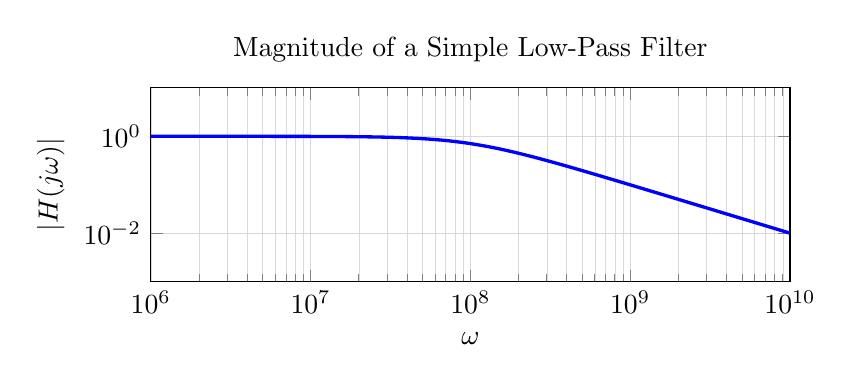
\begin{tikzpicture}[
    declare function={
        mag(\omega)= 1/(sqrt(1 + \omega^2 /10^16));
    }
    ]
    \begin{loglogaxis}
    [
    title={Magnitude of a Simple Low-Pass Filter},
    ymin=0.001, ymax=10, ylabel=$|H(j\omega)|$,
    xmin=10^6, xmax=10^10, xlabel=$\omega$,
    domain=10^6:10^10,
    grid=both, grid style={line width=.1pt, draw=gray!30},
    width=\textwidth * 0.8,
    height=\textwidth / 3,
    samples=100
    ]
    \addplot [blue,very thick] {mag(x)};
    \end{loglogaxis}
    \end{tikzpicture}

    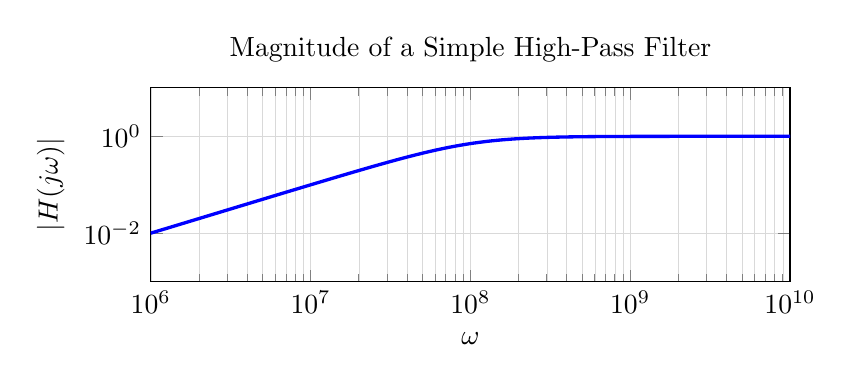
\begin{tikzpicture}[
    declare function={
        mag(\omega)= (\omega/10^8)/(sqrt(1 + \omega^2 /10^16));
    }
    ]
    \begin{loglogaxis}
    [
    title={Magnitude of a Simple High-Pass Filter},
    ymin=0.001, ymax=10, ylabel=$|H(j\omega)|$,
    xmin=10^6, xmax=10^10, xlabel=$\omega$,
    domain=10^6:10^10,
    grid=both, grid style={line width=.1pt, draw=gray!30},
    width=\textwidth * 0.8,
    height=\textwidth / 3,
    samples=100
    ]
    \addplot [blue,very thick] {mag(x)};
    \end{loglogaxis}
    \end{tikzpicture}

    \item \textbf{Phase Response}: We examine the phase response of a system by plotting $\angle{H(\omega)}$ on a semilog scale (where the x-axis is a log scale and the y-axis is a linear scale).

    \begin{tabular}[t]{|c|c|c|c|c|c|}
        \hline
        Type & $\omega < \omega_c / 10$ & $\omega = \omega_c / 10$ & $\omega = \omega_c$ & $\omega = 10\omega_c$ & $\omega > 10\omega_c$ \\
        \hline
        Low-Pass & $\angle{H(\omega)} = 0$ & $\angle{H(\omega)} = -5.7^{\circ}$ & $\angle{H(\omega)} = -45^{\circ}$ & $\angle{H(\omega)} = -84.3^{\circ}$ & $\angle{H(\omega)} = -90^{\circ}$ \\
        \hline
        High-Pass & $\angle{H(\omega)} = 90^{\circ}$ & $\angle{H(\omega)} = 84.3^{\circ}$ & $\angle{H(\omega)} = 45^{\circ}$ & $\angle{H(\omega)} = 5.7^{\circ}$ & $\angle{H(\omega)} = 0$ \\
        \hline
    \end{tabular}

    The linear approximation of a phase plot (for a simple high-pass or low-pass filter) will have 3 sections: it will be flat until $\omega_c / 10$, then go down linearly (from $0$ to $-90^{\circ}$ for a low-pass or $90^{\circ}$ to $0$ for a high-pass) until $10\omega_c$, after which the graph is flat. \\

    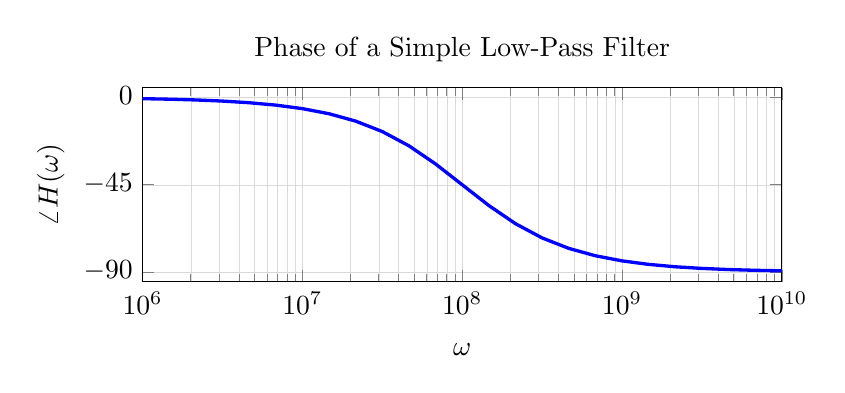
\begin{tikzpicture}[
        declare function={
            ph(\omega)= -atan(\omega/10^8);
        }
    ]
    \begin{semilogxaxis}[
        title={Phase of a Simple Low-Pass Filter},
        typeset ticklabels with strut,
        ymin=-95, ymax=5, ylabel=$\angle H(\omega)$, ytick={-90, -45, 0},
        xmin=10^6, xmax=10^10, xlabel=$\omega$, 
        domain=10^6:10^10, 
        grid=both, grid style={line width=.1pt, draw=gray!30},
        width=\textwidth * 0.8,
        height=\textwidth / 3
    ]
    \addplot [blue,very thick] {ph(x)};
    \end{semilogxaxis}
    \end{tikzpicture}

    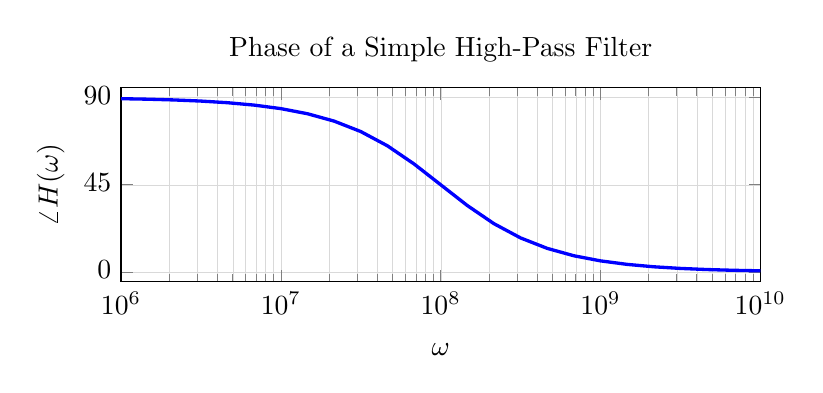
\begin{tikzpicture}[
        declare function={
            ph(\omega)= 90- atan(\omega/10^8);
        }
    ]
    \begin{semilogxaxis}[
        title={Phase of a Simple High-Pass Filter},
        typeset ticklabels with strut,
        ymin=-5, ymax=95, ylabel=$\angle H(\omega)$,
        ytick={0, 45, 90},
        xmin=10^6, xmax=10^10, xlabel=$\omega$,
        domain=10^6:10^10, 
        grid=both, grid style={line width=.1pt, draw=gray!30},
        width=\textwidth * 0.8,
        height=\textwidth / 3
    ]
    \addplot [blue,very thick] {ph(x)};
    \end{semilogxaxis}
    \end{tikzpicture}
\end{enumerate}
\textbf{Higher-order filters} (for instance, a band-pass filter): Consider a transfer function that is the product of multiple first-order transfer functions, for instance:
\begin{align*}
    H(\omega) = \frac{j\omega/\omega_{c1}}{1 + j\omega/\omega_{c1}} \cdot \frac{1}{1 + j\omega/\omega_{c2}}.
\end{align*}
In this case, you can plot the overall transfer function by "adding" the individual first-order plots:
\begin{enumerate}
    \item For magnitude plots, plot the first-order components on a log-log scale, and then add the plots together:
    $$\text{If } H(\omega) = H_1(\omega) \cdot H_2(\omega) \text{, then } \log |H(\omega)| = \log |H_1(\omega)| + \log |H_2(\omega)|.$$

    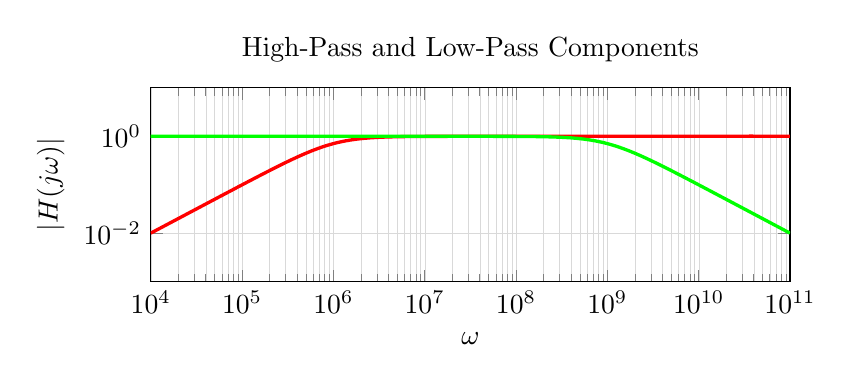
\begin{tikzpicture}[
    declare function={
        mag1(\omega)= (\omega/10^6)/(sqrt(1 + \omega^2 /10^12));
        mag2(\omega)= (1)/(sqrt(1 + \omega^2 /10^18));
    }
    ]
    \begin{loglogaxis}
    [
    title={High-Pass and Low-Pass Components},
    ymin=0.001, ymax=10, ylabel=$|H(j\omega)|$,
    xmin=10^4, xmax=10^11, xlabel=$\omega$,
    domain=10^4:10^11,
    grid=both, grid style={line width=.1pt, draw=gray!30},
    width=\textwidth * 0.8,
    height=\textwidth / 3,
    samples=100
    ]
    \addplot [red, very thick] {mag1(x)};
    \addplot [green, very thick] {mag2(x)};
    \end{loglogaxis}
    \end{tikzpicture}

    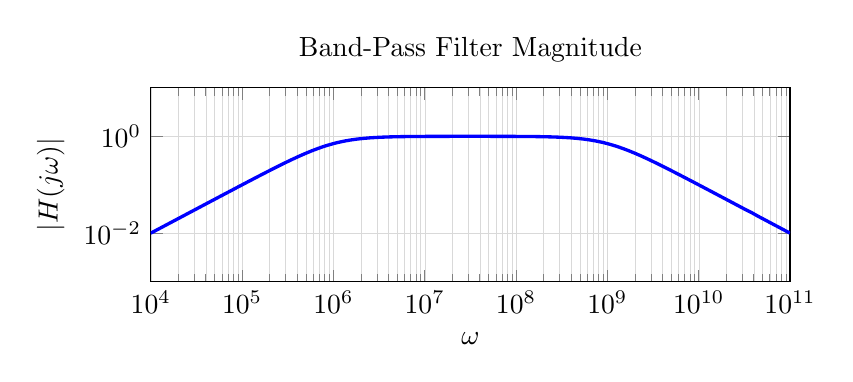
\begin{tikzpicture}[
    declare function={
        mag1(\omega)= (\omega/10^6)/(sqrt(1 + \omega^2 /10^12));
        mag2(\omega)= (1)/(sqrt(1 + \omega^2 /10^18));
    }
    ]
    \begin{loglogaxis}
    [
    title={Band-Pass Filter Magnitude},
    ymin=0.001, ymax=10, ylabel=$|H(j\omega)|$,
    xmin=10^4, xmax=10^11, xlabel=$\omega$,
    domain=10^4:10^11,
    grid=both, grid style={line width=.1pt, draw=gray!30},
    width=\textwidth * 0.8,
    height=\textwidth / 3,
    samples=100
    ]
    \addplot [blue, very thick] {mag1(x) * mag2(x)};
    \end{loglogaxis}
    \end{tikzpicture}
    \item For phase plots, plot the first-order components on a semilog scale, and then add the plots together:
    $$\text{If } H(\omega) = H_1(\omega) \cdot H_2(\omega) \text{, then } \angle{H(\omega)} = \angle{H_1(\omega)} + \angle{H_2(\omega)}.$$

    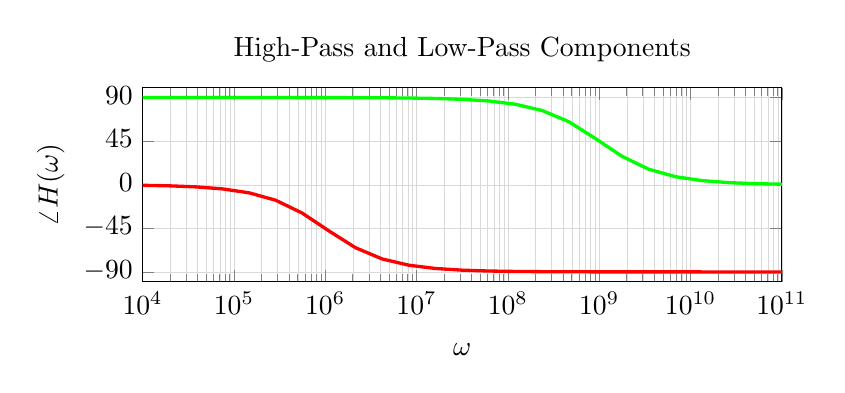
\begin{tikzpicture}[
    declare function={
        ph1(\omega)= -atan(\omega/10^6);
        ph2(\omega)= 90-atan(\omega/10^9);
    }
    ]
    \begin{semilogxaxis}
    [
    title={High-Pass and Low-Pass Components},
    typeset ticklabels with strut,
    ymin=-100, ymax=100, ylabel=$\angle H(\omega)$, ytick={-90, -45, 0, 45, 90},
    xmin=10^4, xmax=10^11, xlabel=$\omega$, 
    domain=10^4:10^11, 
    grid=both, grid style={line width=.1pt, draw=gray!30},
    width=\textwidth * 0.8,
    height=\textwidth / 3
    ]
    \addplot [red, very thick] {ph1(x)};
    \addplot [green, very thick] {ph2(x)};
    \end{semilogxaxis}
    \end{tikzpicture}

    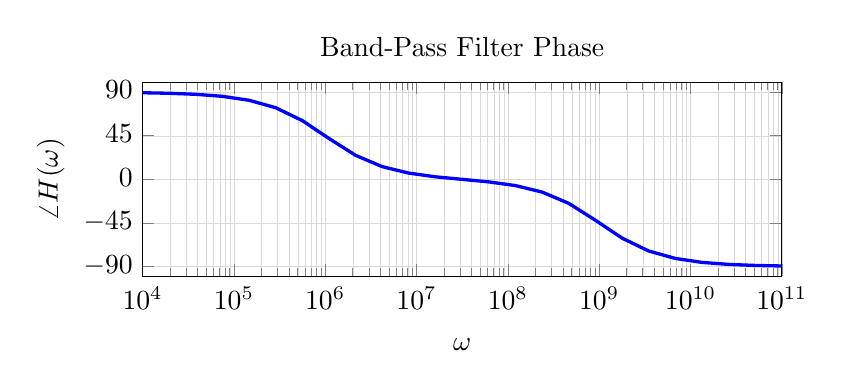
\begin{tikzpicture}[
    declare function={
        ph1(\omega)= -atan(\omega/10^6);
        ph2(\omega)= 90-atan(\omega/10^9);
    }
    ]
    \begin{semilogxaxis}
    [
    title={Band-Pass Filter Phase},
    typeset ticklabels with strut,
    ymin=-100, ymax=100, ylabel=$\angle H(\omega)$, ytick={-90, -45, 0, 45, 90},
    xmin=10^4, xmax=10^11, xlabel=$\omega$, 
    domain=10^4:10^11, 
    grid=both, grid style={line width=.1pt, draw=gray!30},
    width=\textwidth * 0.8,
    height=\textwidth / 3
    ]
    \addplot [blue, very thick] {ph1(x) + ph2(x)};
    \end{semilogxaxis}
    \end{tikzpicture}
\end{enumerate}
As you will see in the next section, you can more easily plot higher-order transfer functions by using the concept of \textbf{poles and zeros}.

\newpage
\subsection*{Poles and Zeros}
You can more easily examine a transfer function by factoring the numerator and denominator to be in the following form:
\begin{align*}
    H(\omega) = K \cdot \frac{(j\omega)^{N_{z0}} (1 + j\omega/\omega_{z1}) (1 + j\omega/\omega_{z2}) \cdots}{(j\omega)^{N_{p0}} (1 + j\omega/\omega_{p1}) (1 + j\omega/\omega_{p2}) \cdots}
\end{align*}
\textbf{Components of this transfer function}:
\begin{enumerate}
    \item $K$: This represents a constant gain.
    \item $(j\omega)^{N_{z0}}$: This represents a \textbf{zero} at the origin. The exponent $N_{z0}$ denotes the \textbf{order} of that zero.
    \item $(1 + j\omega/\omega_{zi})$: This represents a zero at $\omega = \omega_{zi}$.
    \item $(j\omega)^{N_{p0}}$ (on the denominator): This represents a \textbf{pole} at the origin, where $N_{p0}$ is the order of that pole.
    \item $(1 + j\omega/\omega_{pi})$ (on the denominator): This represents a pole at $\omega = \omega_{pi}$.
\end{enumerate}

\textbf{Graphing a transfer function using poles and zeros}: The general idea is to graph the individual poles and zeros, and then add the plots together.

Below, we will be examining a log-log magnitude plot ($\log |H(\omega)|$ versus $\log(\omega)$). Note that this is a linear approximation, not an exact representation of the magnitude:
\begin{enumerate}
    \item Break $H(\omega)$ into a product of poles and zeros.
    \item \textit{Starting out}: 
    \begin{itemize}
        \item If there is a pole at the origin, then the plot starts out by linearly decreasing with a slope (on a log-log plot) of $-N_{p0}$. \item If there is a zero at the origin, then the plot starts out by linearly increasing with a slope of $N_{z0}$.
        \item For either a pole or a zero at the origin, the graph will intersect $\log |H(\omega)| = 0$ at $\omega = 1$.
        \item If you have no poles or zeros at the origin, the graph will start out with a flat line of height $\log |H(\omega)| = 0$.
    \end{itemize}
    \item \textit{Poles and zeros not at the origin}: For this part of the plot, we will look at the poles and zeros in numerical order:
    \begin{itemize}
        \item Whenever you encounter a pole, decrease the slope by 1. For instance, if the plot has been a flat line up until this point, then it will start decreasing with a slope of 1. If it had been increasing until this point with a slope of 1, the plot will be flat after the pole.
        \item When you encounter a zero, increase the slope by 1. For instance, if the plot had been decreasing with a slope of 1 until this point, it will be a flat line after.
        \item Repeat with all poles and zeros.
    \end{itemize}
    \item \textit{Vertical offset}: if there is a gain $K \neq 1$, then shift your entire plot vertically by $\log{K}$.
\end{enumerate}
Note that we will mainly focus on magnitude plots this semester, but you can follow a similar procedure for phase plots. See Discussion 6A for more info. 

\newpage
\subsection*{Resonance}
Consider an LRC circuit in the frequency domain:
\begin{center}
    \begin{circuitikz}
        \draw (0, 2) node[label=left:$V_{in}$] {}
        to [short, -*] (0, 2)
        to[L = $j \omega L$] (2,2)
        to[R = $R$, -*] (4.5, 2)
        node[label=right:$V_{out}$] {};
        \draw (4.5, 2) to[C = $\frac{1}{j \omega C}$] (4.5, 0.5)
        node[ground] {};
    \end{circuitikz}
\end{center}

If our output is the voltage over the capacitor, you can derive the transfer function as follows: \\

First, use the Voltage Divider relation to get the output in terms of the impedances of our circuit elements:
\begin{align*}
    V_{out} = \frac{Z_C}{Z_C + Z_L + Z_R} V_{in} = \frac{\frac{1}{j\omega C}}{\frac{1}{j\omega C} + j\omega L + R} V_{in} \\
    H(j\omega) = \frac{V_{out}}{V_{in}} = \frac{\frac{1}{j\omega C}}{\frac{1}{j\omega C} + j\omega L + R}
\end{align*}
Now, we can manipulate the transfer function so that it's easier to analyze. In this case, we will make the numerator a constant and the denominator a polynomial in terms of $j\omega$. \\

Multiply the numerator and denominator by $j\omega C$:
\begin{align*}
    H(j\omega) = \frac{1}{1 + (j\omega)^2LC + j\omega RC}
\end{align*}
Divide the numerator and denominator by $LC$:
\begin{align*}
    H(j\omega) = \frac{1/LC}{(j \omega)^2 + j \omega R/L + 1/LC}
\end{align*}

We define $\omega_n = \sqrt{1/LC}$ to be the \textit{resonant frequency} of the circuit.
At this frequency, the impedances of the capacitor and inductor ``cancel out'' ($j \omega_n L = \frac{1}{j \omega_n C}$), resulting in a spike in the magnitude of the transfer function.

\begin{align*}
    H(\omega_n = \sqrt{1/LC}) = \frac{1/LC}{j\sqrt{\frac{1}{LC}} \frac{R}{L}}
\end{align*}

For an LRC filter with $\omega_n = 10^4$, the magnitude of the transfer function would look something like below. (\textit{Note: the plot is on a log-log scale.}) \\
\begin{center}
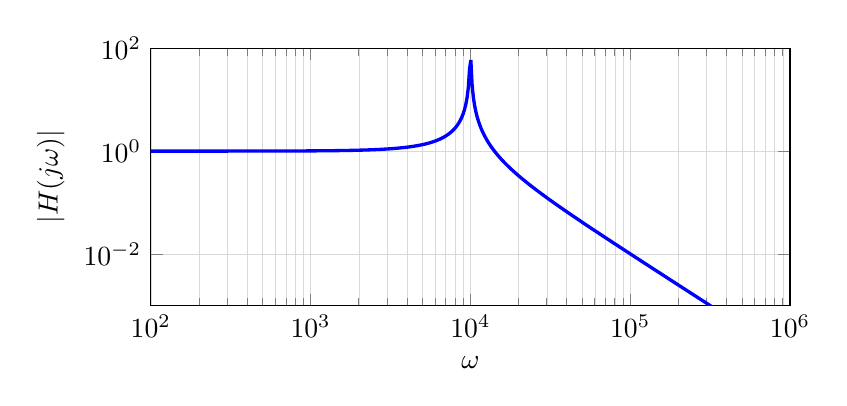
\begin{tikzpicture}[
    declare function={
    mag(\omega)= (10^8) / (sqrt((10^8 - \omega^2)^2 + (\omega * 100)^2))
    ;
    }
]
    \begin{loglogaxis}
    [
    ymin=0.001, ymax=100, ylabel=$|H(j\omega)|$,
    xmin=10^2, xmax=10^6, xlabel=$\omega$,
    domain=10^2:10^6,
    grid=both, grid style={line width=.1pt, draw=gray!30},
    width=\textwidth * 0.8,
    height=\textwidth / 2.5,
    samples=500
    ]
    \addplot [blue,very thick] {mag(x)};
    \end{loglogaxis}
\end{tikzpicture}
\end{center}